\documentclass[border=10pt]{standalone}
\usepackage{luatexja-fontspec}
\usepackage{tikz}
\usetikzlibrary{positioning, arrows.meta, calc}

% ヒラギノ丸ゴシックを指定
\setmainjfont{HiraMaruProN-W4}

\begin{document}
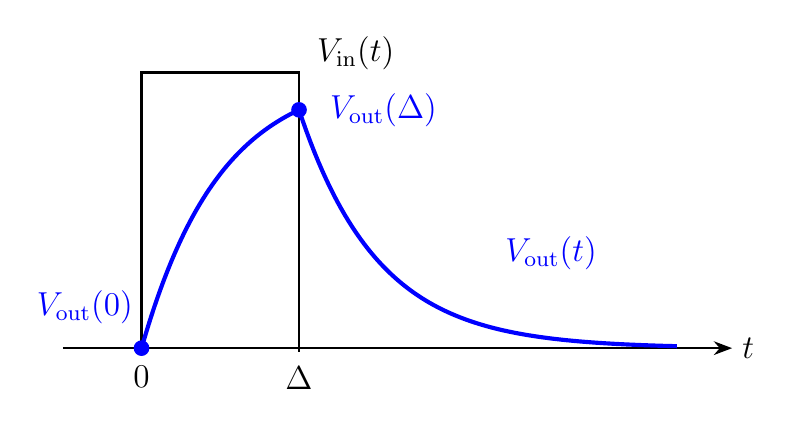
\begin{tikzpicture}[
    thick,                  % 全体の線を太めにする
    >=Stealth,              % 綺麗な矢じりを使用
    font=\large,            % フォントサイズを一括で大きくする
    blue_dot/.style={circle, fill=blue, inner sep=2pt}
]

    % --- 1. 座標軸の描画 ---
    \draw [->] (-1.0, 0) -- (7.5, 0) node[right] {$t$};
    
    % 横軸の目盛りラベル
    \node [below=0.1cm of {0,0}] {$0$};
    \node [below=0.1cm of {2,0}] {$\Delta$};
    \draw (2, 0.05) -- (2, -0.05);

    % --- 2. 入力波形 V_in(t) の描画 ---
    \draw [line width=1.0pt] (0,0) -- (0, 3.5) -- (2, 3.5) -- (2,0);
    % 重なりを防ぐため、矩形の「右上」にテキストを配置
    \node [above right=-0.1cm and 0.1cm of {2, 3.5}] {$V_{\mathrm{in}}(t)$};


    % --- 3. 出力波形 V_out(t) の描画（青い曲線） ---
    \draw [blue, line width=1.5pt, domain=0:2, samples=50] 
        plot (\x, {3.5 * (1 - exp(-\x))});

    \draw [blue, line width=1.5pt, domain=2:6.8, samples=100] 
        plot (\x, {3.5 * (1 - exp(-2)) * exp(-(\x-2))});


    % --- 4. 特徴点の青丸ドットとラベル ---
    % スタート地点 V_out(0)
    \node [blue_dot] (dot0) at (0,0) {};
    \node [blue, above left=0.1cm and -0.1cm of dot0] {$V_{\mathrm{out}}(0)$};

    % ピーク地点 V_out(\Delta)
    \node [blue_dot] (dotDelta) at (2, {3.5 * (1 - exp(-2))}) {};
    % 重なりを防ぐため、ドットの「真右」に配置
    \node [blue, right=0.15cm of dotDelta] {$V_{\mathrm{out}}(\Delta)$};

    % 減衰中のラベル V_out(t)
    \node [blue] at (5.2, 1.2) {$V_{\mathrm{out}}(t)$};

\end{tikzpicture}
\end{document}

\documentclass[border=10pt]{standalone}
\usepackage{luatexja-fontspec}
\usepackage{tikz}
\usetikzlibrary{positioning, arrows.meta, calc}

% ヒラギノ丸ゴシックを指定
\setmainjfont{HiraMaruProN-W4}

\begin{document}
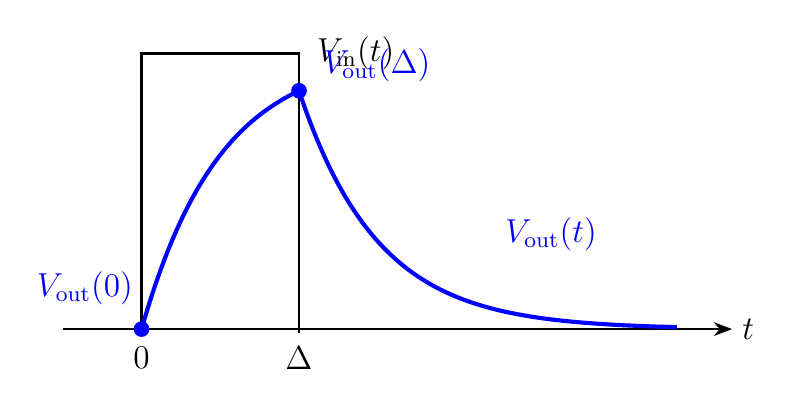
\begin{tikzpicture}[
    thick,                  % 全体の線を太めにする
    >=Stealth,              % 綺麗な矢じりを使用
    font=\large,            % フォントサイズを一括で大きくする
    % 青いドット（注目点）のスタイル
    blue_dot/.style={circle, fill=blue, inner sep=2pt}
]

    % --- 1. 座標軸の描画 ---
    % 横軸（t軸）
    \draw [->] (-1.0, 0) -- (7.5, 0) node[right] {$t$};
    
    % 横軸の目盛りラベル (0 と \Delta)
    \node [below=0.1cm of {0,0}] {$0$};
    \node [below=0.1cm of {2,0}] {$\Delta$};
    % \Deltaの位置にある小さな区切り線
    \draw (2, 0.05) -- (2, -0.05);

    % --- 2. 入力波形 V_in(t) の描画（黒い矩形パルス） ---
    % 0から立ち上がり、\Deltaで立ち下がるパルス
    \draw [line width=1.0pt] (0,0) -- (0, 3.5) -- (2, 3.5) -- (2,0);
    \node [right=0.1cm of {2, 3.5}] {$V_{\mathrm{in}}(t)$};


    % --- 3. 出力波形 V_out(t) の描画（青い曲線） ---
    % [0 から \Delta までの立ち上がり（充電）曲線]
    % 数式: 3.5 * (1 - exp(-x))
    \draw [blue, line width=1.5pt, domain=0:2, samples=50] 
        plot (\x, {3.5 * (1 - exp(-\x))});

    % [\Delta 以降の立ち下がり（放電）曲線]
    % 数式: 3.5 * (1 - exp(-2)) * exp(-(x-2))
    \draw [blue, line width=1.5pt, domain=2:6.8, samples=100] 
        plot (\x, {3.5 * (1 - exp(-2)) * exp(-(\x-2))});


    % --- 4. 特徴点の青丸ドットとラベル ---
    % スタート地点 V_out(0)
    \node [blue_dot] (dot0) at (0,0) {};
    \node [blue, above left=0.1cm and -0.1cm of dot0] {$V_{\mathrm{out}}(0)$};

    % ピーク地点 V_out(\Delta)
    % 数式から計算される t=2 のときの高さ（約3.03）にドットを配置
    \node [blue_dot] (dotDelta) at (2, {3.5 * (1 - exp(-2))}) {};
    \node [blue, above right=-0.1cm and 0.1cm of dotDelta] {$V_{\mathrm{out}}(\Delta)$};

    % 減衰中のラベル V_out(t)
    \node [blue] at (5.2, 1.2) {$V_{\mathrm{out}}(t)$};

\end{tikzpicture}
\end{document}
